\section{WC 10/3/25}

\subsection*{Overview:}
This week I didn't have quite as much extra time to work on my EPQ due to volunteering commitments each evening however I still have some achievements to document. I had previously ensured this time was marked as less intensive in my project plan so I could focus on my extracurricular commitments.

\subsection*{Achievements, Thoughts and Ideas:}


On Monday I started working on the whiteboard editor, once again implementing it from my previous prototype made during the research phase. Unfortunately I faced some similar issues as I did with the document editor such as incorrect connections between different technologies now that I am using a fronted library (Vue JS). Having learnt the benefits of starting afresh from last time I took this path again. This time however I noticed that from the start I was facing the same challenges as with my prior code:

\begin{figure}[H]
    \centering
    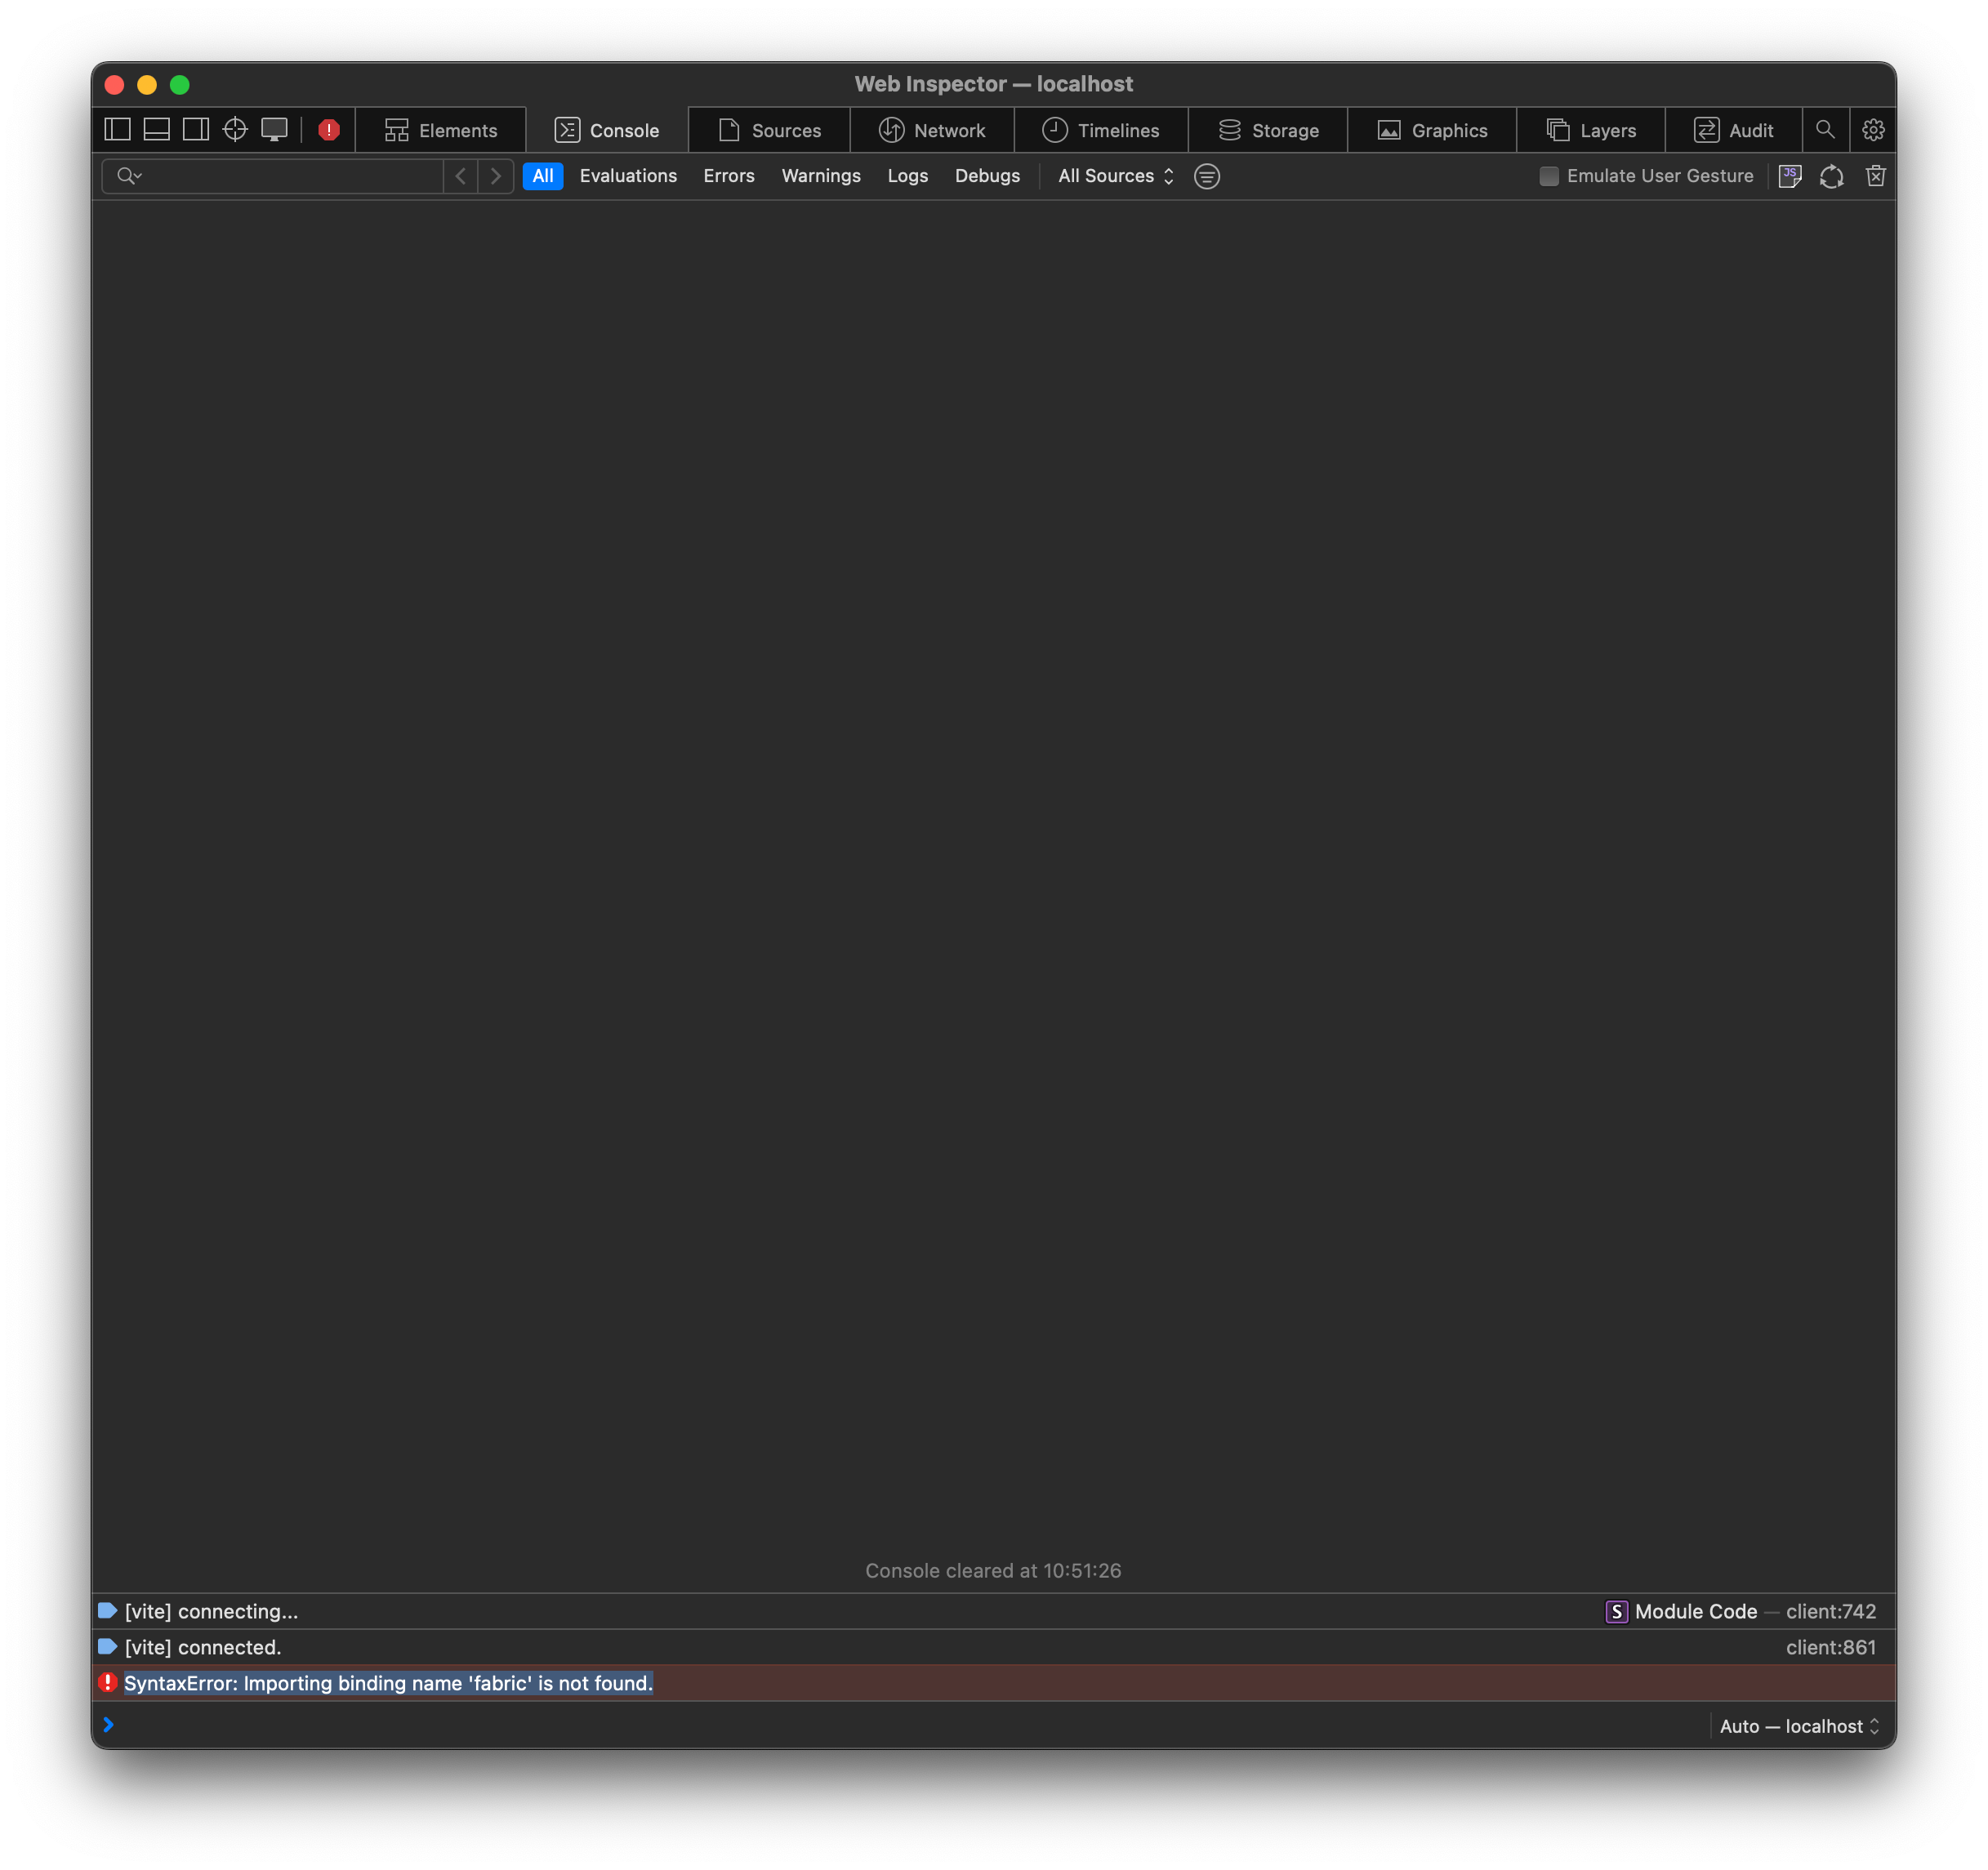
\includegraphics[width=0.8\textwidth]{Diary/21_WC_10-3-25/media/consoleError.png}
    \caption{Console Error when trying to run the whiteboard editor}
\end{figure}


Having done some quick research I found that the Fabric Js library I had used in my prototypes earlier this year had since had some notable upgrades and improvements that would enable me to more easily add features such as context aware erasing and multimedia support. Although this means I am going to update my understanding of fabric I suspect this will result in a better end product despite the new learning I will have to do.

The above slowed down my development of the whiteboard tool, and so I'm going to need to spend next week finishing up this part of my software. 

Whilst I didn't manage to complete the Fabric Js implementation I did add a couple more features to last weeks' document editor such as more in depth weblinks.


During lessons this week I worked on my Project plan, establishing the features I want to build during my time on my EPQ journey.



\subsection*{Power of Three:}
\textbf{This week's Tasks laid out per day}

\begin{tabularx}{\textwidth}{
  >{\raggedright\arraybackslash}X  % First column expands
  >{\centering\arraybackslash}p{1.5cm}  % Middle column has fixed width
  >{\raggedright\arraybackslash}X  % Third column expands
}
\toprule
\textbf{Goal} & \textbf{Achieved?} & \textbf{Notes} \\
\midrule


\rowcolor{gray!10}
\multicolumn{3}{l}{\textbf{Monday}} \\
Build Login Backup system (implementing prior prototype)  & \ding{51} & \\
Restructure prototype code for Implementation & \ding{51} & \\


\rowcolor{gray!10}
\multicolumn{3}{l}{\textbf{Thursday}} \\
Develop Whiteboard editor UI & \ding{51} & Further research required\\
Develop Whiteboard editor Features& \ding{55} & " \\



\rowcolor{gray!10}
\multicolumn{3}{l}{\textbf{Friday}} \\
Create Project outcome plan & \ding{51} & Please find here: \nameref{projectChoice:ProjectOutcomePlan}\\

\bottomrule
\end{tabularx}

\subsection*{What went well?}
The technology I am using for my whiteboard tool has had some very positive updates which will make my final implementation easier and more feature rich.

\subsection*{Plans for next week:}
Learn more about the Fabric Js updates and how to implement them most effectively. Finish the whiteboard tool and start integrating both editors into the main application.
